\documentclass{article}
\usepackage[margin=1.6cm]{geometry}
\usepackage{amsmath,graphicx,booktabs}
\begin{document}
\section*{Post hoc bounded bias--variance control}
All three known Phase C graphs were retained for structural coverage, with no screening on favorable outcomes. The two endpoint noise rates $p=0.001,0.02$, all three Richardson orders, and the noisy baseline were evaluated at $B=1024$ shots per grid point. This new $12\times12$ finite grid is not the archived $120\times120$ campaign; weighted gamma is treated as a prescribed finite domain, without asserting periodicity. Each configuration has 500 independent multinomial landscape replicates, with independent points, scales and methods. No campaign-level endpoint is retested here.

For objective $C=-\mathrm{cut}$ and scale $j$, the exact density distribution gives $\mu_j=E[C_j]$ and $v_j=E[C_j^2]-\mu_j^2$. Integer shot allocation is the existing largest-remainder allocation proportional to absolute Richardson weights. Thus
\[b(\theta)=\sum_jw_j\mu_j(\theta)-C_0(\theta),\qquad V(\theta)=\sum_j\frac{w_j^2v_j(\theta)}{n_j},\qquad E[(\widehat C-C_0)^2]=b^2+V.\]
We average these quantities over the grid. Regret is measured at the selected grid minimum using the exact ideal landscape, normalized by its range. The exact mean landscape isolates residual deterministic distortion, while finite-shot selection includes sampling. A preregistered-for-this-control contrast compares the row-major ideal minimum with the smallest strictly positive ideal gap (tolerance $10^{-10}$); it is illustrative rather than a worst-case competitor. The protocol file predates execution, but this entire control remains post hoc relative to the original campaign.

\begin{center}\scriptsize
\begin{tabular}{lllrrrrr}\toprule
Graph & $p$ & Method & Bias$^2$ & Variance & Expected MSE & Mean regret & MC regret\\\midrule
G1\_C4 & 0.001 & noisy & 5.641e-05 & 0.001276 & 0.0013324 & 2.961e-16 & 7.508e-16 \\
G1\_C4 & 0.001 & linear & 2.9491e-08 & 0.0050927 & 0.0050927 & 2.961e-16 & 6.857e-16 \\
G1\_C4 & 0.001 & quadratic & 2.0227e-11 & 0.015553 & 0.015553 & 2.961e-16 & 7.597e-16 \\
G1\_C4 & 0.001 & cubic & 5.0075e-13 & 0.045554 & 0.045554 & 2.961e-16 & 7.147e-16 \\
G1\_C4 & 0.02 & noisy & 0.01744 & 0.0011817 & 0.018622 & 0 & 7.384e-16 \\
G1\_C4 & 0.02 & linear & 0.0023365 & 0.0046103 & 0.0069468 & 0 & 7.307e-16 \\
G1\_C4 & 0.02 & quadratic & 0.00037661 & 0.013746 & 0.014123 & 0 & 7.461e-16 \\
G1\_C4 & 0.02 & cubic & 6.6847e-05 & 0.039335 & 0.039402 & 0 & 7.869e-16 \\
G2\_weighted4 & 0.001 & noisy & 5.9086e-05 & 0.0010409 & 0.0011 & 0 & 0.001476 \\
G2\_weighted4 & 0.001 & linear & 6.1884e-08 & 0.0041667 & 0.0041668 & 0 & 0.006763 \\
G2\_weighted4 & 0.001 & quadratic & 9.0118e-11 & 0.012772 & 0.012772 & 0 & 0.01635 \\
G2\_weighted4 & 0.001 & cubic & 1.2659e-12 & 0.037572 & 0.037572 & 0 & 0.03866 \\
G2\_weighted4 & 0.02 & noisy & 0.016347 & 0.0010576 & 0.017405 & 0 & 0.003365 \\
G2\_weighted4 & 0.02 & linear & 0.0036086 & 0.0042313 & 0.0078399 & 0 & 0.008734 \\
G2\_weighted4 & 0.02 & quadratic & 0.00095696 & 0.012957 & 0.013914 & 0 & 0.01883 \\
G2\_weighted4 & 0.02 & cubic & 0.0002822 & 0.038064 & 0.038346 & 0 & 0.03222 \\
G3\_weighted6 & 0.001 & noisy & 0.00012843 & 0.0024107 & 0.0025392 & 0 & 2.661e-16 \\
G3\_weighted6 & 0.001 & linear & 1.6207e-07 & 0.0096309 & 0.009631 & 0 & 0.0006944 \\
G3\_weighted6 & 0.001 & quadratic & 2.4845e-10 & 0.029448 & 0.029448 & 0 & 0.006533 \\
G3\_weighted6 & 0.001 & cubic & 2.8021e-12 & 0.08638 & 0.08638 & 0 & 0.03498 \\
G3\_weighted6 & 0.02 & noisy & 0.034029 & 0.0023194 & 0.036348 & 0 & 2.751e-16 \\
G3\_weighted6 & 0.02 & linear & 0.0085711 & 0.0091993 & 0.01777 & 0 & 0.002257 \\
G3\_weighted6 & 0.02 & quadratic & 0.0025529 & 0.027942 & 0.030495 & 0 & 0.01204 \\
G3\_weighted6 & 0.02 & cubic & 0.00082951 & 0.081509 & 0.082338 & 0 & 0.04134 \\
\bottomrule\end{tabular}\end{center}
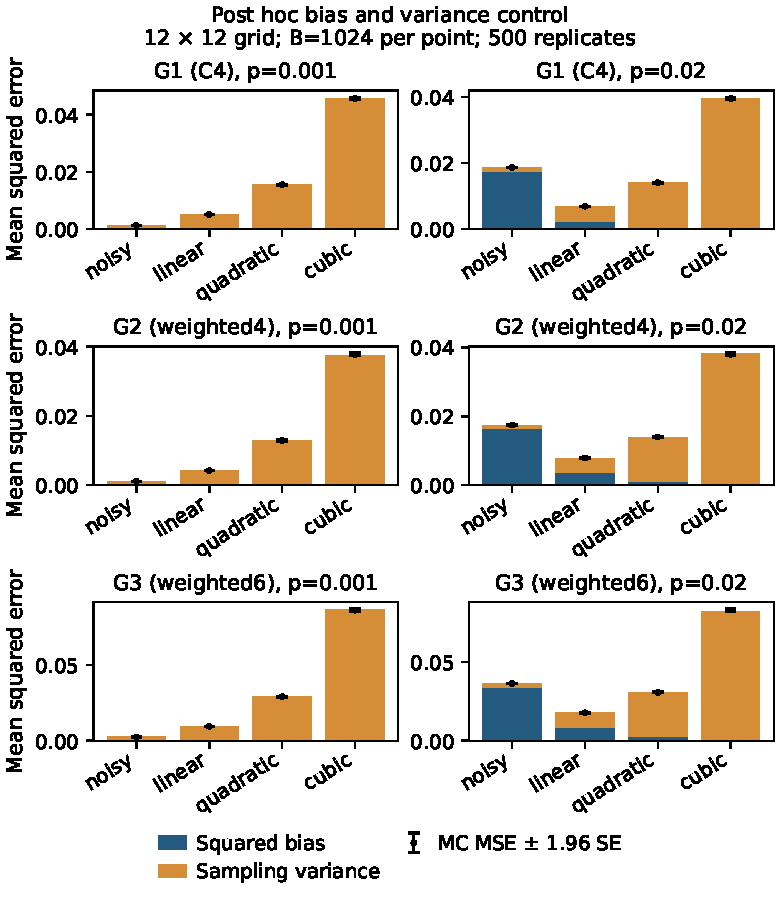
\includegraphics[width=\linewidth]{bias_variance.pdf}
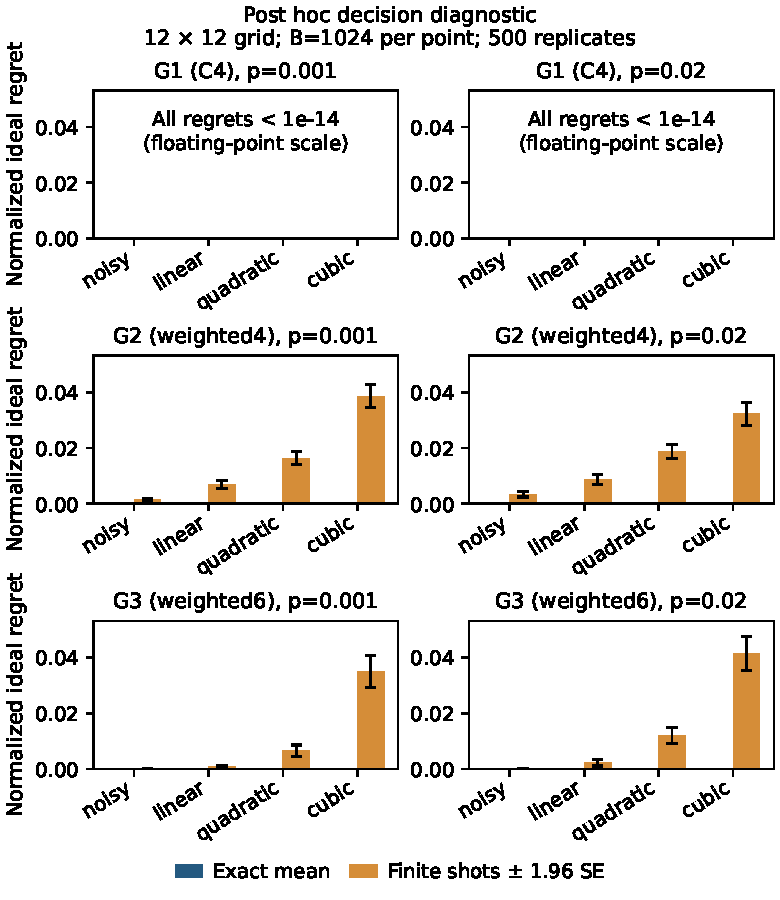
\includegraphics[width=\linewidth]{decision_regret.pdf}

At $p=0.02$, linear and quadratic mitigation reduce expected grid-mean MSE on all three graphs: their MSE ratios to the noisy baseline are respectively $0.373$--$0.489$ and $0.758$--$0.839$. Cubic mitigation increases it ($2.116$--$2.265$), despite lowering squared bias. At $p=0.001$, all orders increase MSE, with ratios of about $3.79$--$3.82$, $11.60$--$11.67$, and $34.02$--$34.19$. Actual sampling-variance ratios are approximately $3.90$--$4.00$, $11.63$--$12.27$, and $33.29$--$36.09$; they need not equal the constant-variance amplification factors $4,12.25,36$ because scale-dependent physical variances and integer allocations enter the exact formula.

All exact mean landscapes select an ideal minimum, up to floating-point differences below $10^{-14}$ in normalized regret. This small grid therefore provides no observed deterministic argmin error, although deterministic pointwise bias remains. For the weighted graphs, finite-shot mean regret is higher with mitigation in every examined configuration; at $p=0.02$ this coexists with lower expected MSE for the first two orders. Sampling is necessary for these observed selection errors, but its effect can interact with residual bias through the decision margins; no counterfactual isolates a pure variance effect here. G1 finite-shot regrets are also below $10^{-14}$, so the decision plot uses one common vertical scale rather than magnifying roundoff. An independent statevector calculation agrees with all 432 ideal grid values to within $6.22\times10^{-15}$; there are 32, 2, and 2 ideal minimizers on G1, G2, and G3 within absolute objective tolerance $10^{-10}$. A reversal against one fixed ideal minimizer need not cause selection of a suboptimal grid point: another equivalent ideal minimizer can win. The chosen contrast is not a substitute for the full selection calculation. Zero empirical errors among 500 replicates do not imply zero population error probability.

The plotted MC error bars are descriptive $1.96$ standard errors over independent landscape replicates, not simultaneous confidence intervals or tests of cross-method differences. All 24 MC MSE estimates lie within $1.919$ estimated standard errors of their exact expectations. Exact mean and second moments were checked against Aer at two preselected points (maximum discrepancies $2.73\times10^{-14}$ and $1.33\times10^{-13}$ respectively); source hashes, software versions, timings, all pointwise values, and replicate outcomes are supplied. The production calculation took 69.3 seconds on this machine, below the declared 600-second bound. Small-grid observations do not identify the mechanism of every archived discordant cell, and the single selected contrast cannot characterize the full argmin competition.
\end{document}
